% !TeX spellcheck = en_US
\documentclass[]{upb_cs_thesis} % include german inside brackets for a German thesis

% load your own packages and user-defined commands
\usepackage{amsmath, amssymb, amsfonts}% mathematical symbols and the like
\usepackage{amsthm}% definitions, theorems, etc.
\usepackage[colorinlistoftodos]{todonotes}% marking open todos in text/on margins
\usepackage{subfig}% multi-part figures with separate captions per part
\usepackage{url}% render URLs correctly and make them clickable through the hyperref package
\usepackage{longtable}% tables that span multiple pages
\usepackage{booktabs}% tables that actually look good
\usepackage{acronym}% consistently use acronyms
\usepackage{algorithm}
\usepackage[noend]{algpseudocode}
\usepackage[scaled=0.85]{beramono}
\usepackage{listings}
\lstset{language=SQL,morekeywords={PREFIX,java,rdf,rdfs,url}}
\usepackage[export]{adjustbox}
%\usepackage[automake]{glossaries} %Load glossaries package
\usepackage{array}
\usepackage{makecell}
\usepackage{graphicx}
\usepackage{capt-of}
\usepackage{placeins}
%%%%%%%%%
% Some commands for setting up theorem environments as provided by package 
% amsthm --- language sensitive
%%%%%%%%%
\theoremstyle{plain}
\newtheorem{definition}{Definition}[chapter]
\newtheorem{lemma}[definition]{Lemma}
\ifgerman
	\newtheorem{theorem}[definition]{Satz}
	\newtheorem{corollary}[definition]{Korollar}
	\newtheorem{example}[definition]{Beispiel}
\else
	\newtheorem{theorem}[definition]{Theorem}
	\newtheorem{corollary}[definition]{Corollary}
	\newtheorem{example}[definition]{Example}
\fi



%%%%%%%%%
% Your commands should go here...
%%%%%%%%%
\newcommand*{\eg}{e.\,g.}
\newcommand*{\ie}{,i.\,e.,}
\newcommand*{\cf}{c.\,f.}
\newcommand*{\etal}{et~al.}
\newcommand\subfigWidth{0.5}
\newcommand\subfigCurvePlotWidth{0.5}
\newcommand\tp{\textit{transitive path} }
\newcommand\tps{\textit{transitive paths} }
\newcommand\tpsp{\textit{transitive paths}. }
\newcommand\dtp{\textit{direct transitive path} }
\newcommand\dtpp{\textit{direct transitive path}. }
\newcommand\dtps{\textit{direct transitive paths} }
\newcommand\dtpsp{\textit{direct transitive paths}. }

\newcommand{\GGRP}{$Graph_{GRP}$}
\newcommand{\DGRP}{$Dict_{GRP}$}
\newcommand{\GHDT}{$Graph_{HDT}$}
\newcommand{\DHDT}{$Dict_{HDT}$}

\newcommand{\CR}[1]{$CR_{#1}$}
\newcommand{\CRDict}[1]{$CR_{Dict_{#1}}$}
\newcommand{\CRGraph}[1]{$CR_{Graph_{#1}}$}

\renewcommand\theadalign{bc}
\renewcommand\theadfont{\bfseries}
\renewcommand\theadgape{\Gape[4pt]}
\renewcommand\cellgape{\Gape[4pt]}


\newacro{template}[UPB-CS-TT]{Paderborn University Computer Science thesis template}

\DeclareMathOperator{\testop}{top}



% set up some resources (graphics and bibliography)
\graphicspath{{figures/}}


%%%%%%%%%
% your thesis title, name, advisor, etc. go here;
%%%%%%%%%
\title{Grammar-based Compression of RDF Graphs}
\author{Philip Frerk}
\thesistype{Master's Thesis}
%\thesistype{Bachelor's Thesis}
%\thesistype{Masterarbeit}
%\thesistype{Bachelorarbeit}
\degree{Master of Science (M.Sc.)}
%\degree{Bachelor of Science}
\researchgroup{Data Science}
\supervisor{Prof. Dr. Axel-Cyrille Ngonga Ngomo}
\submissiondate{\today}

\setlength{\parindent}{0pt}


% here your thesis really starts
\begin{document}

% start with the titlepage, the formalities, and then the abstract
% This file defines the title page of your thesis. You typically do not need to
% edit it. It is language sensitive and prints arguments passed to commands
% \author, \title, \thesistype, \degree, \researchgroup, \supervisor and
% \submissiondate, where required.
\begin{titlepage}
	\begin{center}
		\begin{minipage}{135mm}
			\hbadness=10000
			
\includegraphics[height=30mm]{figures/uni-logo}\\
			\ifgerman
				\textsf{
					\hspace*{20mm} Fakultät für Elektrotechnik,
					Informatik und Mathematik \\
					\hspace*{20mm} Institut für Informatik \\
					\hspace*{20mm} Arbeitsgruppe \theresearchgroup{} \\
				}
			\else
				\textsf{
					\hspace*{20mm} Faculty for Computer Science, 
					Electrical Engineering and Mathematics \\
					\hspace*{20mm} Department of Computer Science \\
					\hspace*{20mm} Research Group \theresearchgroup{} \\
				}
			\fi 
		\end{minipage}\\[40pt]

		{\huge \thethesistype{}}\\[5pt]
		\ifgerman
			Gerichtet an die Arbeitsgruppe \theresearchgroup{}\\
			zur Erreichung des Grades\\[5pt]
		\else
			Submitted to the \theresearchgroup{} Research Group\\
			in Partial Fullfilment of the Requirements
			for the Degree of\\[5pt]
		\fi 
		{\huge \thedegree{} (M.Sc.)}\\[30pt]

		{\Huge\textbf{\thetitle{}}}\\[30pt]

		\ifgerman
			von\\
		\else
			by\\
		\fi 
		{\Large\textsc{\theauthor{}}}\\[60pt]
		
		Thesis Advisor:\\[8pt]
		
		{\large Michael Röder, M.Sc.}\\[30pt]

		\ifgerman
			Betreut durch:\\
		\else
			Thesis Supervisors:\\[8pt]
		\fi 
		{\large \thesupervisor{}}\\[5pt]
		
		\ifgerman
		Betreut durch:\\
		\else
	    
		\fi 
		{\large Prof. Dr. Stefan Böttcher}\\[30pt]

		Paderborn, \thesubmissiondate{}
	\end{center}
\end{titlepage}
 % prints the title page
% This is the legal statement
%  - that your thesis is a work of your own,
%  - that you have not used any source other than the ones you mention, 
%  - that you genuinely created your theses to achieve the desired academic
%    degree, and have not presented it to another examination board; and
%  - that you have clearly marked all concepts and ideas that you have adopted
%    from other works.
\chapter*{Erklärung}
	\thispagestyle{empty}
	Ich versichere, dass ich die Arbeit ohne fremde Hilfe und ohne
	Benutzung anderer als der angegebenen Quellen angefertigt habe und dass
	die Arbeit in gleicher oder ähnlicher Form noch keiner anderen
	Prüfungsbehörde vorgelegen hat und von dieser als Teil einer
	Prüfungsleistung angenommen worden ist. Alle Ausführungen, die wörtlich
	oder sinngemäß übernommen worden sind, sind als solche
	gekennzeichnet.\\
	\vspace{27pt}

	\begin{center}
		\begin{tabular}{l p{0.1\textwidth} r}
			\cline{1-1} \cline{3-3}
			\begin{minipage}[t]{0.4\textwidth}
				\centering
				Ort, Datum
			\end{minipage}
			&&  
			\begin{minipage}[t]{0.4\textwidth}
				\centering
				Unterschrift
			\end{minipage}
	\end{tabular}
\end{center}

 % prints the statement that you worked on your own and did not commit plagiarism
%\cleardoublepage
\vspace*{\fill}
%\begin{abstract}
%	We present a full documentation of the \ac{template} and how to use it.
This document also serves as a demonstrator to show what documents
\ac{template} produces.
Have fun!

%\end{abstract}
\acresetall
\vspace*{\fill}
\emptypage

%\setcounter{secnumdepth}{2}
%\setcounter{tocdepth}{1}
\tableofcontents % prints the table of contents


%%%%%%%%%
% the contents of your thesis go into file body.tex
%%%%%%%%%
% !TeX spellcheck = en_US
\chapter{Introduction}\label{ch:introduction}

\section{Motivation}
The majority of data on the Internet is unstructured because it is mainly text. That makes it difficult for machines to extract knowledge from the data and answer specific queries. In the context of the Semantic Web, an attempt is made to build a knowledge base using structured data. Here the data is stored as graphs. A graph is an often used data structure which consists of nodes and edges. The edges connect the different nodes. This thesis will focus on knowledge graphs, which are about expressing knowledge or facts. A possible format for the such graphs is the Resource Description Framework (RDF)\footnote{\label{foot:2}https://www.w3.org/RDF/}, in which a graph is represented by triples of the form $ (subject, predicate, object) $, where $ subject $ and $object$ are nodes and $predicate$ is an edge of the graph. A triple is typically used to express a certain fact. \todo{hier noch genauer, was die einzelnen Komponenten sind}

In reality, such knowledge graphs can become very large with millions or even billions of nodes and edges. \todo{hier evtl Beispiele von knowledge bases} The following three use cases can then become very slow or even infeasible: storage, transmission and processing. Therefore we are looking for a method to compress knowledge graphs. 

The current most popular compressor for RDF data is HDT~\cite{hdt}. Here the data is made smaller by a compact representation of the triples. HDT is explained in more detail in chapter ~\ref{related_work_hdt}.

The task of this thesis is to compare HDT with a grammar-based compression. As the name suggests, such a compression is based on the principle of a formal grammar, with productions that can be nested among each other. There are not yet many grammar-based compression algorithms for graphs. One of the best known is GraphRePair~\cite{maneth}. This is a compressor that works for any type of graph and is therefore also applicable for RDF. Why the algorithm is particularly suitable for RDF is explained in chapter~\ref{related_work_grammar_based}.

It will be examined for which use cases which of the two approaches is more suitable. What these use cases are is explained in more detail below.



\section{General Idea}

%We will first explain roughly how grammar-based compression works. The details of the algorithm are explained in detail in chapter~\ref{ch:related_work}.
%
%A compression algorithm in general tries to find patterns in data that occur multiple times. Since we are interested in graphs here, these patterns consist of nodes and edges (and their labels). A grammar-based algorithm works as follows: 
%
%\begin{enumerate}
%	\item Search for a pattern $p$ occurring most often.  (Terminate if there is no pattern $p$ occurring more than once.)
%	\item Replace all occurrences of $p$ with a non-terminal $N_p$, store $p$ only at one place and let $N_p$ reference to $p$.
%	\item Go to step 1.
%\end{enumerate}
%
%In this way, the graph becomes smaller as you remove more redundancy. At the same time, no information is lost because the non-terminals are references the original data. The compression can therefore be completely reversed if that is desired. Also, querying is possible on the compressed graph since all information is still contained in it.

As already mentioned, there are essentially three use cases for RDF data:

\begin{enumerate}
	\item Storage
	\item Transmission
	\item Processing/Consumption
\end{enumerate}

The idea is that you can make all these use cases easier / possible by compression, especially if you are dealing with very large amounts of data. In the first two use cases, compression can be helpful by reducing the size of the data. Thus the data can be stored more compactly and above all can be transferred faster, which occurs frequently in reality and can become a problem due to possibly slow transfer speeds \todo{here possibly concrete numbers}.

The third use case (Processing/Consumption) is about reading or writing access to data. The more common case of read access is typically the execution of queries on RDF data. For example, you want to find out which other nodes a given node is connected to. But there are other examples which will be explained in the course of the thesis. A compression algorithm can help in this respect by making it possible to answer such queries directly on the compressed graphs. This may even be faster than on the original data due to the reduced size.

The aim of the thesis is to compare the two compressors (HDT and GRP) with regard to these use cases and finally determine which approach works better for which use cases.



\section{Thesis Structure}
\todo{machen}

% !TeX spellcheck = en_US
\chapter{Related Work}\label{ch:related_work}

This chapter gives an introduction to the domain RDF and introduces the different compression algorithms discussed in this thesis.

\section{RDF}\label{sec:rdf}

RDF is a format for structured data on the web. It can be formally described as follows. Let the following sets be infinite and mutually disjoint:

\begin{itemize}
	\item $U$ (URI references, typically represent unique entities or properties)
	\item $B$ (Blank nodes, represent an arbitrary value, necessary for displaying more complex logical statements)
	\item $L$ (Literals, represent fixed values, e.g. numbers or strings)
\end{itemize}

An RDF triple $(s,p,o) \in (U \cup B) \times U \times (U\cup B \cup L)$ displays the statement that the subject $s$ is related to the object $o$ via the predicate $p$. So a subject can anything but a literal. A predicate can only be a URI and an object can be anything.

\section{HDT}\label{related_work_hdt}

HDT~(\cite{hdt}) is the best known approach to compressing RDF data because it is directly tailored to RDF. The idea behind it is to make RDF's extensive representation more compact, thus reducing memory size. In the normal RDF format  (e.g. turtle), each triple is written down after another. This does not only require much space, but is also not good for query performance, since each single triple has to be traversed within a query execution.

It is easy to see that a more compact representation can be achieved by cleverly grouping the triples. That is exactly what HDT does. Imagine for example some triples that all have the same subject $s$. These would then be written in turtle format as follows:

\begin{align*}
(s,p_1,o_{11}),...,(s,p_1,o_{1_{n1}}),(s,p_2,o_{2_1}),...,\\
	(s,p_2,o_{2_{n2}}),...,(s,p_k,o_{kn_k})
\end{align*}

In HDT the triples are then grouped by $s$.

\begin{align*}
s \to [(p_1,(o_{1_1},...,o_{1_{n_1}})),(p_2,(o_{2_1},...,o_{2_{n_2}})),...,\\
 (p_k , (o_{k_{n_k}} ))]
\end{align*}

Since all triples have the same subject $s$, it does not have to be written down at the beginning of each triple anymore. On the second level the triples are then grouped according to the predicates. So all triples with the predicate $p_1$ come first, then all with the predicate $p_2$ and so on. Finally only the different objects have to be enumerated since the subject and predicate are already implicitly given. You will now see how HDT implements this mechanism.

First, all URIs and literals (which are usually quite long) are mapped to unique IDs (integers). From now on these IDs will be used. You can see the triples with the IDs in Fig.~\ref{fig:hdt_overview} on the left ('Plain Triples'). 

The above mentioned grouped representation is called 'Compact Triples' and can be seen in Fig.~\ref{fig:hdt_overview} in the middle. In the array 'Predicates' you can see the IDs of the predicates. A '0' means that from now on a new subject comes. For example, the first two entries in the 'Predicates' are linked to the first subject, since there is a '0' in the third position in the array. 

This works analogously for the objects, in the array 'Objects' the IDs of the objects are listed, and a '0' here means that from then on a new predicate comes. For instance, the first entry in 'Objects' is a '6', so the first derived triple would be $(1,2,6)$. The second entry of 'Objects' is a '0' since there is a change from predicate '2' to '3' in 'Predicates'.

The last representation of triples is called 'Bitmap Triples'.  This is a slight adaption of 'Compact Triples'. The array $S_p$ has the same content as 'Predicates', but without the zeros. That job is done by the bit-array $B_p$ in which a '1' at position $i$ means that at position $i$ in $S_p$ there comes a change of the subject (this change was previously denoted by a '0' in 'Predicates'). 

That works analogously for the objects where $S_o$ has the same content as 'Objects', but without zeros.

The advantage of 'Bitmap Triples' is that queries can be executed faster on this representation. Also, the compressed size is slightly smaller than with 'Compact Triples'. Therefore, 'Bitmap Triples' are always used in the current version of HDT.

HDT has also procedures for answering queries, but those will not be mentioned here, because they are not relevant for the thesis.~\cite{hdt}

\begin{figure}[h]
	\centering
	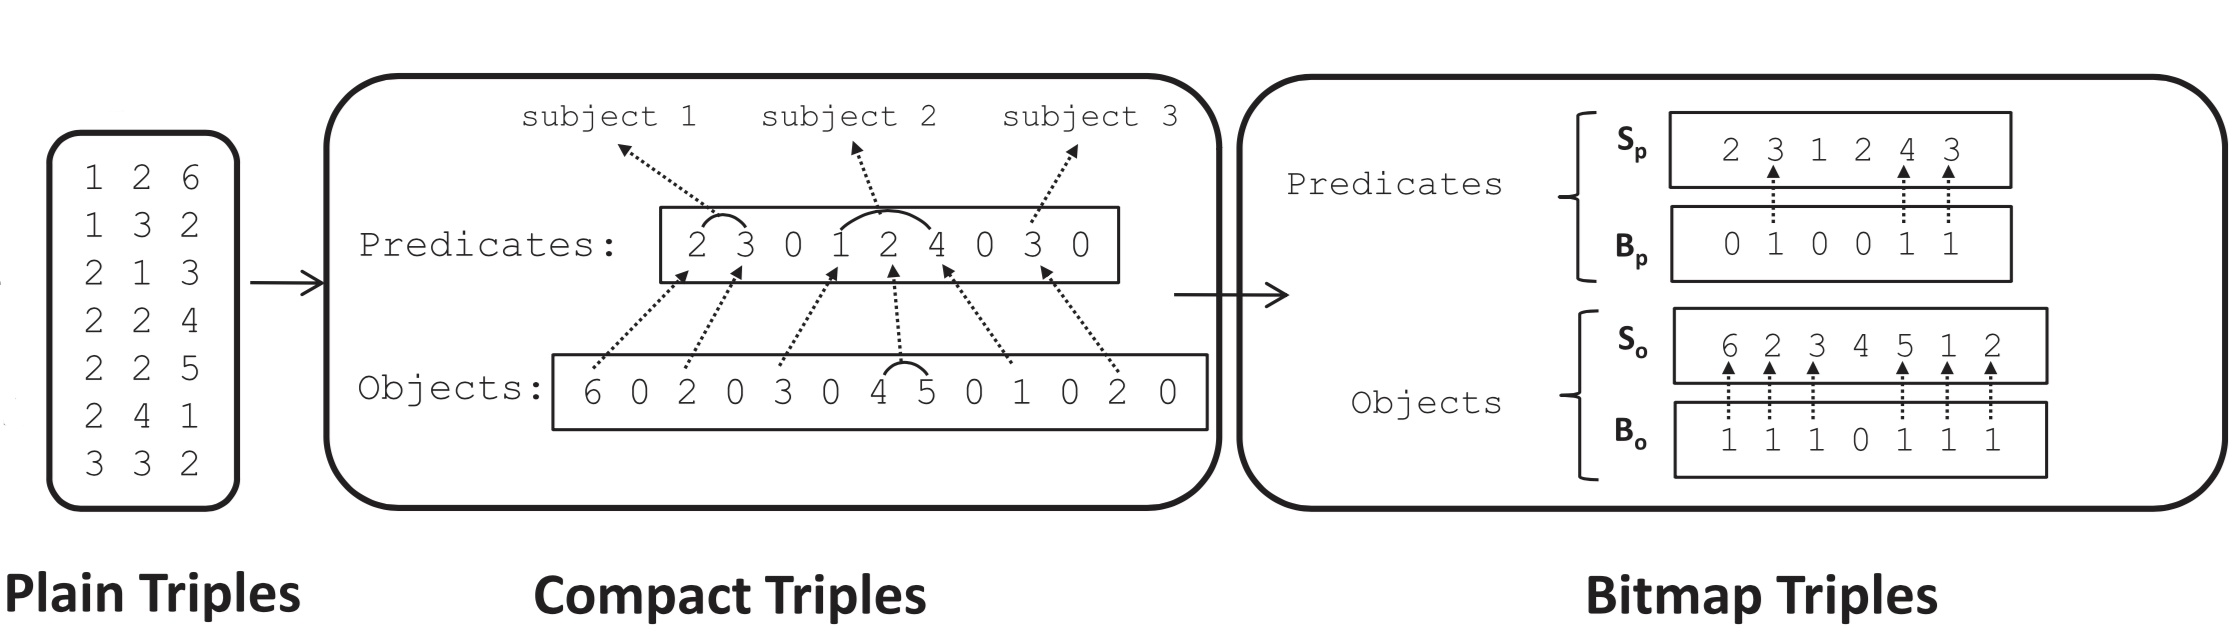
\includegraphics[width=1\textwidth]{figures/relatedwork/hdt1}
	\caption{Three different representations of triples in HDT}
	\label{fig:hdt_overview}
\end{figure}


\section{Grammar-based Graph Compression}\label{related_work_grammar_based}

In this section we will discuss two different approaches to grammar-based graph compression. First, ~\cite{mattdk} is introduced and briefly explained why the approach is less suitable for this thesis. Then~\cite{maneth}, which the thesis will focus on, is introduced.

\subsection{Dürksen's Algorithm}

An approach to grammar-based compression of graphs was developed in~\cite{mattdk}. Here the authors assume a hyper graph with node and edge labels. Such a graph can be seen in Fig.~\ref{fig:transformation} on the left. To simplify the compression, a so-called transformation is now executed, in which a new node is inserted for each edge $e$, which then has the same label as $e$. The original structure of the graph is obtained by connecting two nodes, which were previously connected by an edge, indirectly by the new node. The result of the transformation is a graph, which only has node labels, but no edge labels. Moreover, hyper edges (edges with more than two incident nodes) are no longer present due to the transformation.

\begin{figure}[h]
	\centering
	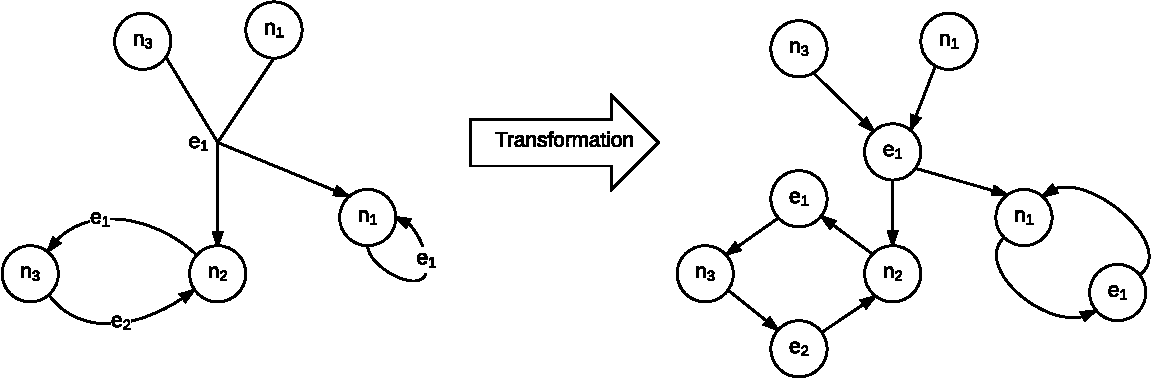
\includegraphics[width=1\textwidth]{figures/relatedwork/transf}
	\caption{Transformation of a labeled graph (each edge is replaced by a new node having the label of the replaced edge).}
	\label{fig:transformation}
\end{figure}

Thus patterns like in Fig.~\ref{fig:basicdigram} can be replaced. Here it happens twice that a node with the label \textit{X} is connected with a node with the label \textit{Y}. This pattern is then stored in a central location and can be referenced via the label \textit{X'}. Thus only two nodes remain in the compressed graph (with \textit{X'} as label) and the graph was reduced to a smaller size. There are some details which make  this pattern replacement possible, but they are neglected at this point.

Dürksen's algorithm does not seem to be suitable for RDF, because it is based on the fact that there are several nodes with the same label. However, since in RDF a node represents an entity that normally does not occur twice, Dürksen's basic assumption is not fulfilled in RDF.

In addition, Dürksen's algorithm is not yet in a mature state, i.e. there is only a rudimentary implementation that does not work reliably for large graphs. In addition, work is currently underway to find a compact representation of such a compressed graph in order to save the data with little memory.~\cite{mattdk}

For these reasons we will focus on the compressor GraphRePair, which is presented in chapter~\ref{ch:GRP}.

\begin{figure}[h]
	\centering
	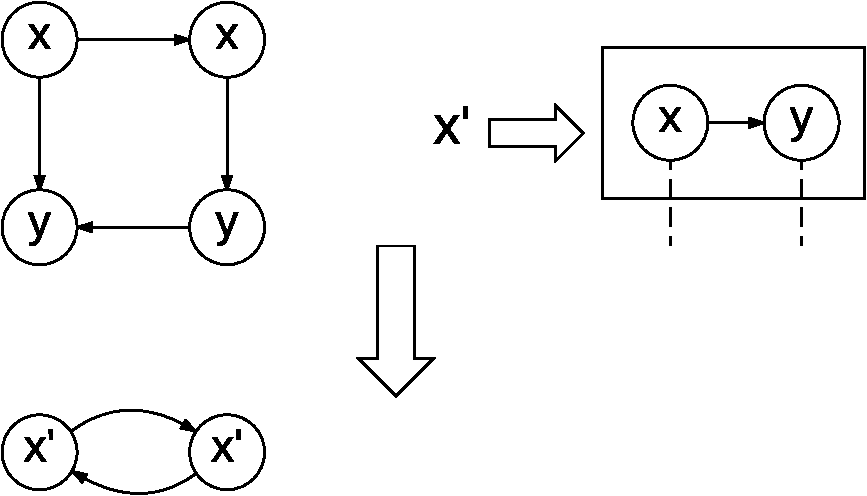
\includegraphics[width=0.6\textwidth]{figures/relatedwork/basisdigram}
	\caption{Replacement of two occurrences of the pattern $X \to Y$ by nodes with the label $X'$.}
	\label{fig:basicdigram}
\end{figure}

\subsection{GraphRePair}\label{ch:GRP}

This chapter deals with GraphRePair, the compressor from~\cite{maneth}. 

\subsubsection{Foundations}

\begin{itemize}
	%\item For a natural number $n\in \mathbb{N}$,  $[n]=\{1,...,n\}$ is defined as the set of all natural numbers from 1 to $n$
	\item For a set $M$, $M^+=\{x_1 \cdot x_2 \cdot ... \cdot x_n | x_1,x_2,..,x_n \in M \}$ is defined as the set of all non-empty strings of $M$ where $\cdot$ stands for the concatenation of two symbols.
	$M^*=M^+ \cup \{ \epsilon \} $ is similar to $M^+$, but it also includes the empty string $\epsilon$ 
	\item 
\end{itemize}


A hypergraph over $\Sigma$ is a tuple $g=(V,E,att,lab,ext)$ where $V=\{1,...,n\}$ is the set of nodes. $E \subseteq \{(i,j) | i,j\in V\} $ is the set of edges. $att: E \to V^+$ is the attachment mapping, $lab: E\to \Sigma$ is the edge label mapping, and $ext \in V^*$ is a series of external nodes.

%The rank of an edge $e$ is defined as $rank(e)=|att(e)|$.

A hypergraph does not contain multi-edges, which means for two edges $e_1\not=e_2$ it holds $att(e_1)\not=att(e_2) \vee lab(e_1)\not=lab(e_2)$. 

For a hypergraph $g=(V,E,att,lab,ext)$  $V_g, E_g, att_g, lab_g, ext_g$ are used to refer to its components.

An example for a hypergraph is illustrated in Fig.~\ref{fig:hypergraph}. Formally the graph can be described as $V=\{1,2,3\}$, $E=\{e_1,e_2,e_3\}$, $att=\{e_1 \mapsto 1 \cdot 2, e_2 \mapsto2 \cdot 3, e_3 \mapsto 2 \cdot 1 \cdot 3 \}$, $lab=\{ e_1\mapsto a, e_2 \mapsto b, e_3 \mapsto A \}$ and $ext=3 \cdot 1$.

\begin{figure}
	\centering
	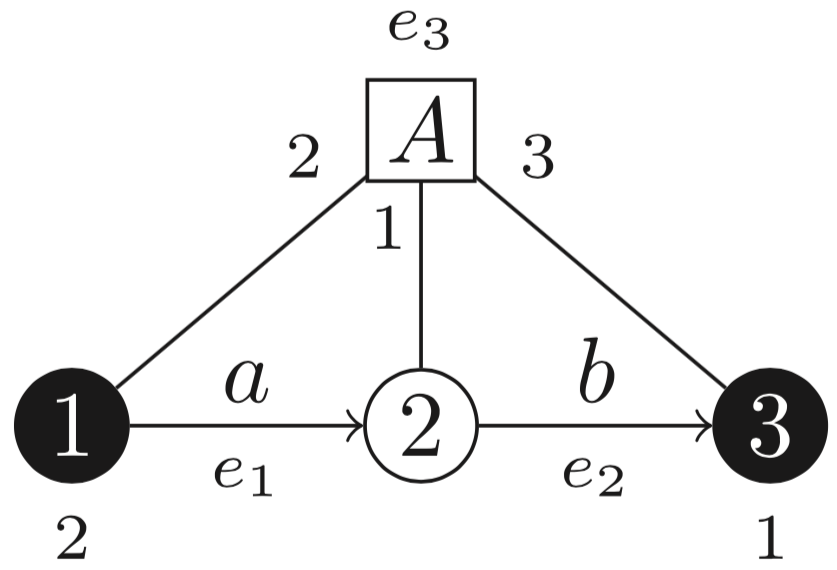
\includegraphics[width=0.3\linewidth]{figures/relatedwork/hypergraph}
	\caption{}
	\label{fig:hypergraph}
\end{figure}

External nodes are black and the numbers below them indicate indices for their position in $ext$. Analogously,  hyper edges ($e_3$ in this case) have indices indicating the order of the attached nodes.~\cite{maneth}

\subsubsection{Digram}

Digrams are like patterns, the same digram can occur multiple times in a graph. Based on that, GRP reduces a graph's size.

A digram $d$ is a hyper graph with $E_d=\{e_1,e_2\}$ so that the following conditions hold:

\begin{enumerate}
	\item $\forall v \in V_d : v\in att_d(e_1) \vee v \in att_d(e_2)$
	\item $\exists v\in V_d : v\in att_d(e_1) \wedge v\in att_d(e_2)$
	\item $ext_d \not= \epsilon$
\end{enumerate}

Condition 1 ensures that all nodes in $d$ are incident to one of the two edges of $d$. Conditions 2 is used to make sure that there is one 'middle node' incident to both edges of $d$. Finally, condition 3 ensures that there are external nodes.~\cite{maneth}


\subsubsection{Digram Occurrence}

Let $g$ be a hyper graph and $d$ be a digram with the two edges $e_1^d,e_2^d$. Let $o=\{e_1,e_2\} \subseteq E_g$ and let $V_o$ be the set of nodes incident with edges in $o$. Then $o$ is an occurrence of $d$ in $g$ if there exits a bijection $b:V_o \to V_d$ so that for $i\in \{1,2\} $ and $v\in V_o$ all following conditions hold:

\begin{enumerate}
	\item $b(v)\in att_d(e_i^d) \text{ iff } v\in att_g(e_i)$
	\item $lab_d(e_i^d)=lab_g(e_i)$
	\item $b(v)\in ext_d \text{ iff } v\in att_g(e) \text{ for some } e\in E_g \setminus o$
\end{enumerate}

Condition 1 and 2 ensure that the two edges of $o$ form a graph isomorphic to $d$. Condition 3 makes sure that every external node of $d$ is mapped to a node in $g$ that is incident to at least one edge in $g$ that is not contained in $o$.~\cite{maneth}

\subsubsection{Algorithm}

Algorithm~\ref{alg:GRP} is the main routine of GraphRePair. The algorithm take a graph as input and returns a grammar whereas $N$ is the set of non terminals, $P$ is the set of productions and $S \in P$ is the start production. It maintains a list of digram occurrences in $g$. As long as this list contains multiple occurrences for one digram the loop will continue. In the loop, the most frequent digram is found and then replaced and the grammar is extended. After a digram replacement the occurrence list has to be updated, because the graph has now changed and former digram occurrences may not exist anymore. Moreover, new digram occurrences can be present now. This occurrence update is a complex process and will not be discussed here, since it is not relevant for the thesis.~\cite{maneth}

\begin{algorithm}
	\caption{GraphRePair (Graph $g=(V,E,att,lab,ext)$)}\label{alg:GRP}
	\begin{algorithmic}[1]
		\State $ N,P\leftarrow \emptyset$
		\State $S \leftarrow g$
		\State $L(d) \leftarrow $ list of non-overlapping occurrences of every digram $d$ appearing in $g$
		\While{$|L(d)|>1$ for at least one digram $d$}
			\State $mfd \leftarrow$ most frequent digram
			\State $A \leftarrow$ new non terminal for $mfd$
			\State Replace every occurrence of $mfd$ in $g$
			\State $N \leftarrow N \cup \{A\}$
			\State $P\leftarrow P\cup \{A \to mfd \}$
			\State Update the occurrence list $L$
		\EndWhile
		\State \Return Grammar $G=(N,P,S)$
	\end{algorithmic}
\end{algorithm}


\subsubsection{Grammar Encoding}

After GRP has constructed a grammar for some graph, this grammar has to be stored in an efficient way. The start production (the graph) is most often much bigger than the other productions and is therefore encoded differently. 

The start production is encoded using $k^2$ trees which is illustrated in Fig.~\ref{fig:encoding}. 

First the matrix is extends with zeros to the next power of two. Then it is partitioned into $k^2$ equally large partitions ($k=2$ here).

The tree's root now represents the whole matrix and its child order correspond to the order of the just created partitions. If a partition only contains zeros, a zero leaf is added to the tree (e.g. in Fig.~\ref{fig:encoding} (a), partition 4, right bottom). Otherwise a one-node is added and the corresponding condition will be partitioned itself. The recursive procedures continues until there is zero-leaf for each path of the tree.

Afterwards, the tree is represented by bit-strings.

Since the graph has also edge labels, an adjacency matrix and its corresponding tree will be created for each of those labels.

\begin{figure}
	\centering
	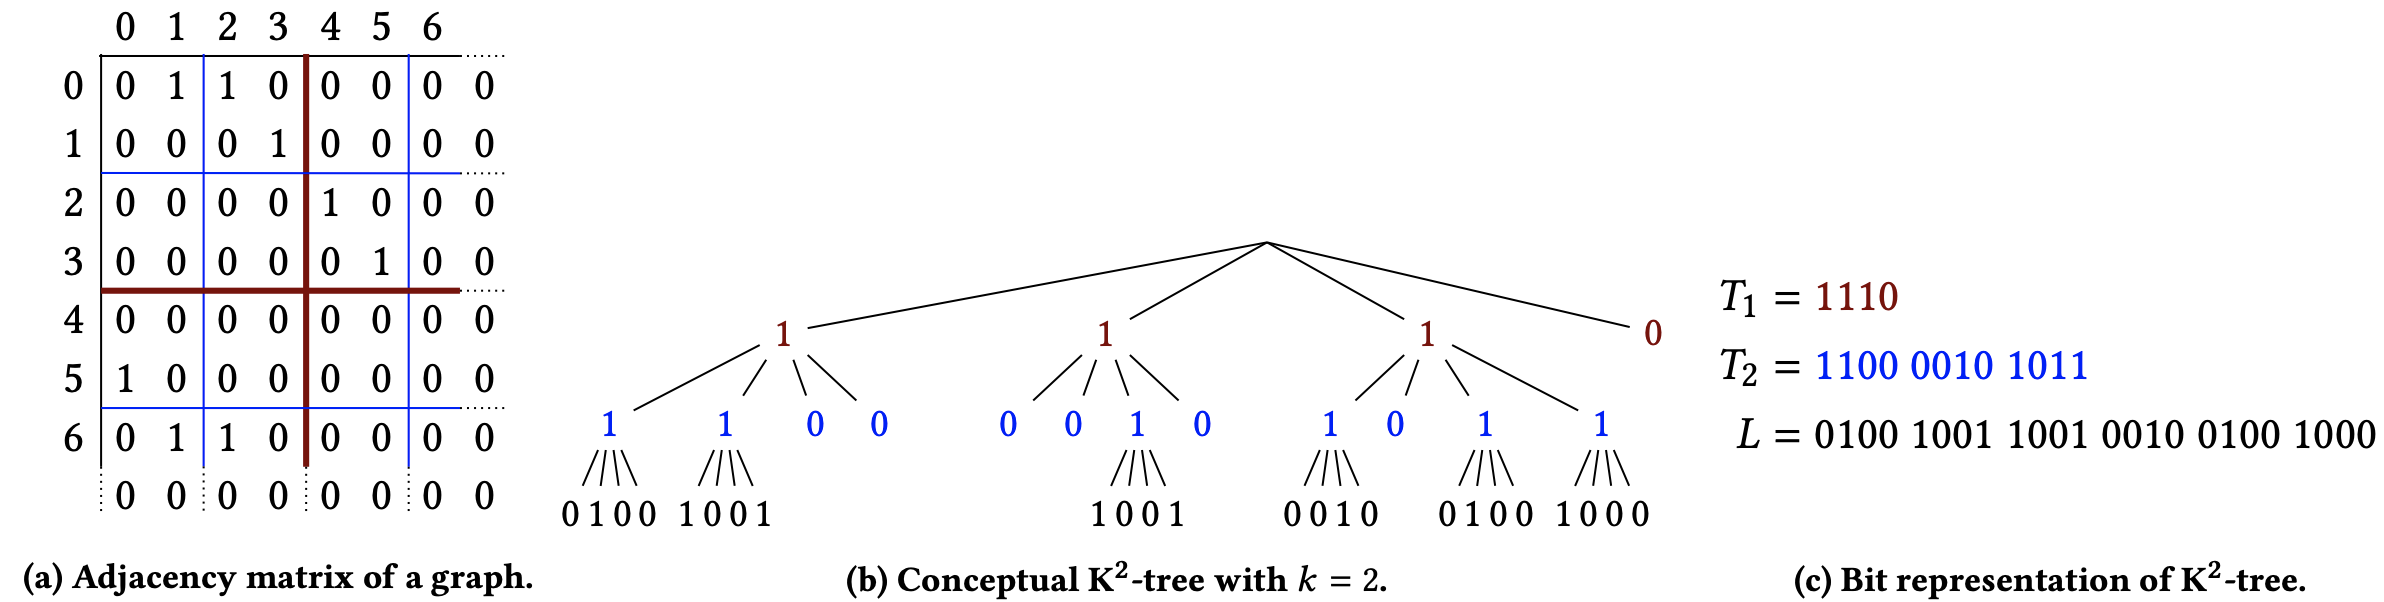
\includegraphics[width=1\linewidth]{figures/relatedwork/encoding}
	\caption{An adjacency matrix, its $k^2$ tree representation and the tree's bit representation.}
	\label{fig:encoding}
\end{figure}


The remaining productions of the grammar are encodes differently, because they are usually quite small compared to the start production. Here so-called $\delta $-codes with variable length are used. Essentially this is a way of displaying numbers as a bit-string in an efficient way (similar to a Huffman Code). To realize that, the right hand side of the components of the production have to represented by numbers, e.g. the edges labels, the node IDs etc.




















% !TeX spellcheck = en_US
\chapter{Approach}\label{ch:approach}

This chapter deals with the derivation of the solution approach for the comparison of the compression algorithms HDT and GraphRePair. First we will introduce some definitions and then we will discuss the concept of the solution approach.

\section{Definitions}

This chapter includes some basic definitions that will be used in the thesis.

\subsection{Compression Ratio}

One of the key metrics for a compressor is its compression ratio. The compression ratio depends on the input data and is defined as follows

\begin{align*}
	\text{compression ratio} = \dfrac{\text{compressed size}}{\text{original size}} \in (0,1]
\end{align*}

The compression ratio is typically in the $(0,1]$ interval, since the compressed data will not be larger than the original data (there are cases where this happens, but it does not happen in the compressors considered here). Obviously, the compressed data cannot have a size of 0 or less.

Normally the compression ratio is measured at the file size level (in byte). If a different measure is used, it will be mentioned at that point.

\subsection{(De-)Compression Time}

Another key metric of a compressor is its (de-)compression time. This metric also depends on the input data and indicates the run time needed for compression and decompression of the data, respectively. The run time is typically measured in milliseconds.

\section{Concept}

Fig.~\ref{fig:benchmark_overview} shows the aspects of a benchmark of two compressors. There are parameters that can be set during the evaluation (they start with $p$) and measures that represent the performance of the algorithms (they start with $m$).

The compressors get an input $p_{input}$, which in this case is in RDF graph. They each produce an output $m_{output}$, the compressed data. For compression and decompression there will be run times, which we call $m_{runtime} $. In addition, there are certain parameters $p_{alg}$ that can be set in the algorithms that change the behavior of the algorithm. \todo{hier kommt noch nicht performance von queries vor}

\begin{figure}[h]
	\centering
	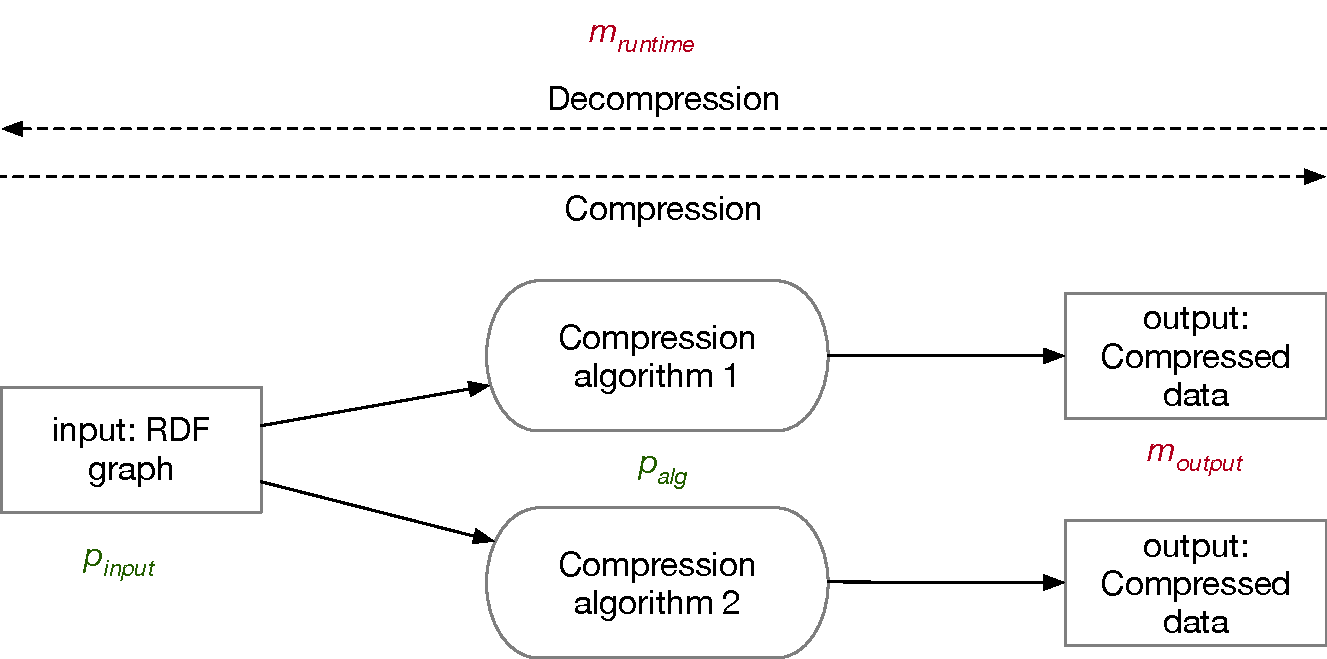
\includegraphics[width=1\textwidth]{figures/approach/Benchmark}
	\caption{The different aspects of a compression process. $p_{input},p_{alg}$ are parameters that can be changed. $m_{output},m_{runtime}$ are measures of the algorithm's performance.}
	\label{fig:benchmark_overview}
\end{figure}



% !TeX spellcheck = en_US
\chapter{GraphRePair vs HDT}\label{ch:GRPvsHDT}

This chapter deals with the comparison between HDT and GRP. The main aim is to determine which of the two compressors achieves a lower compression ratio.

In Ch.~\ref{sec:theory} some basic concepts of the compressors will be discussed again and hypotheses will be made how the compression rate behaves in relation to a certain structuring of RDF data. 

In Ch.~\ref{sec:data_creation} it will be considered how data can be generated that is structured in the way stated in Ch.~\ref{sec:theory}.

Finally in Ch.~\ref{sec:evalHDT} an empirical evaluation of the compression ratios for HDT and GRP for that synthetic RDF data will be done. The evaluation will show that the hypotheses stated in Ch.~\ref{sec:theory} are correct.

\section{Theory}\label{sec:theory}
The obvious question is now whether there are certain properties/features that an RDF graph can have, and which have a positive or negative impact on the compression ratio of one or both algorithms. 

\subsection{Relation between data structure and compression ratio}

First these features are considered for HDT. Fig.~\ref{fig:hdt_overview_1} is shown again. There you can see that the size of the data becomes smaller if there are only a few subjects. This is the case because the bit-array $B_p$ contains a 1 every time a new subject is considered. For example, if there is only one subject, then $B_p$ consists only of zeros.

\begin{figure}[h]
	\centering
	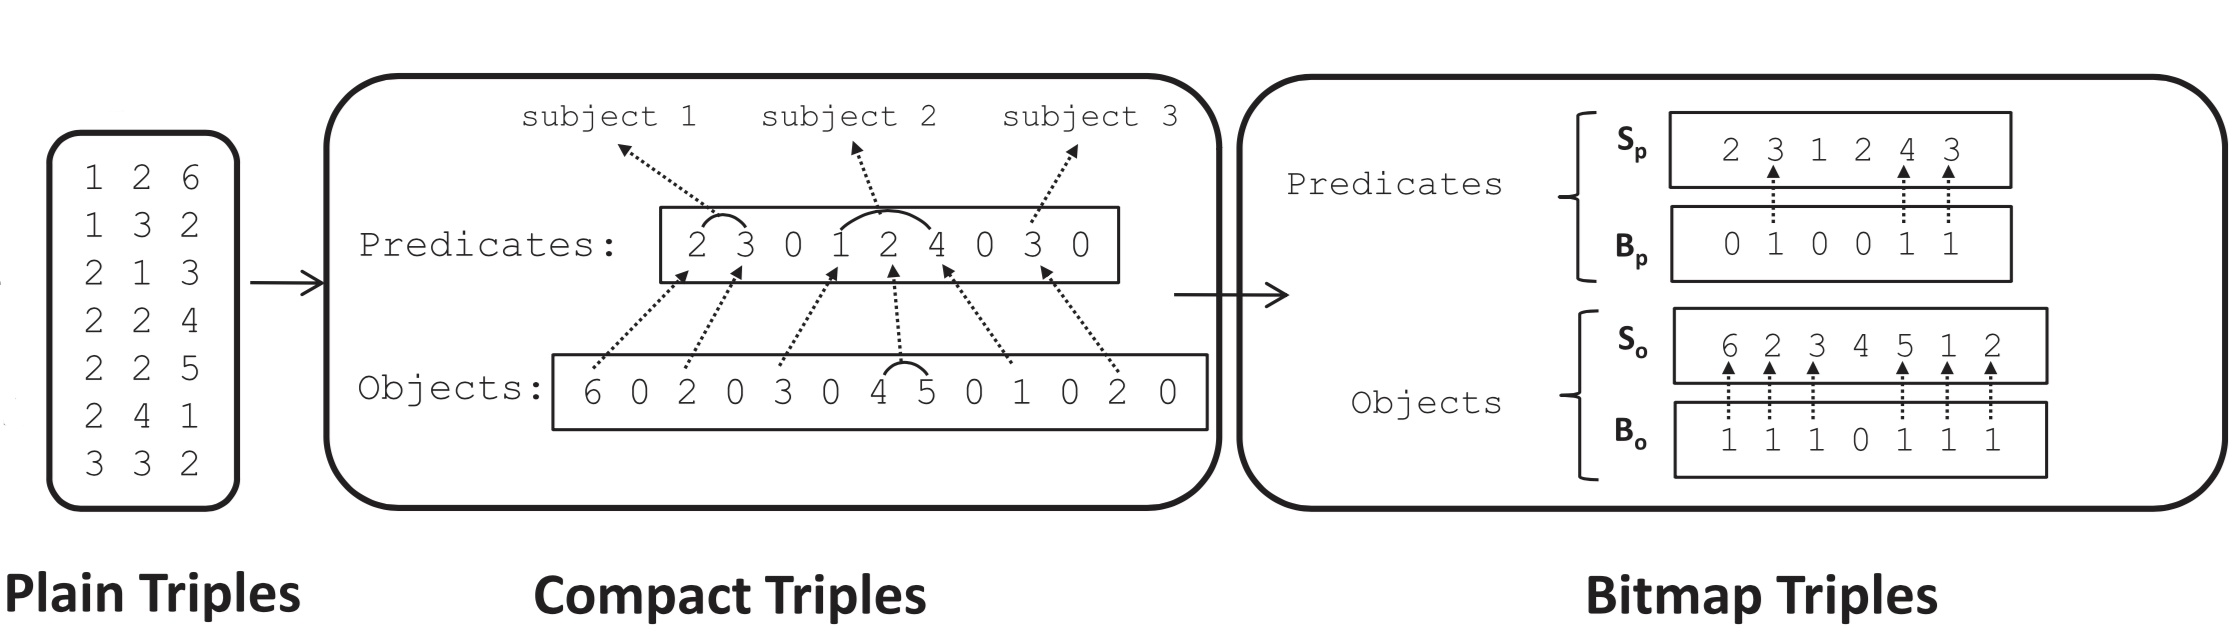
\includegraphics[width=1\textwidth]{figures/relatedwork/hdt1}
	\caption{Three different representations of triples in HDT}
	\label{fig:hdt_overview_1}
\end{figure}

For GRP that feature analysis is more complex. Since GRP constructs grammar rules by using the graph's structure, it is more dependent on the data's structure than HDT. There can be many features that can lead to different constructible grammar rules. Those will not be discussed here. But a simple insight is that GRP's compression ratio will be bigger when there are more different predicates in the graph. This is true, because GRP's grammar rules are based on the repeating edge labels. That fact will be considered in the evaluation.

\subsection{Dictionary Size}

As already explained in Ch.~\ref{ch:related_work}, HDT divides an RDF file into its header, dictionary and triples component. This partially also true for GRP except that GRP does not create a header. But it also assigns an ID to every URI or literal and then only works with these IDs. Unfortunately the authors of~\cite{maneth} did not work on efficient storing of the dictionary. In GRP the size for the dictionary component is just ignored. Therefore we have to add this size in order to compare GRP with HDT in a fair way. To achieve that we just add the same size to the compressed size of GRP that HDT would need to store the dictionary.

\section{Synthetic Data Creation}\label{sec:data_creation}

As has just explained, HDT can compress a graph that is similar to a hub pattern (few subjects, many objects) very well. So it gets worse the further away the graph is from this pattern. This corresponds to the authority pattern, where there are few objects but many subjects.

The task now is to create a series of RDF graphs that first correspond to the hub pattern and then continue to change in the direction of the authority pattern. This is illustrated in Fig.~\ref{fig:star_pattern}. In this scenario all graphs ($G_1$ to $G_m$) have the same size, i.e. the same number of nodes and edges. $G_1$ has only one subject connected to all objects. $G_2$ then has two subjects more and correspondingly 2 objects less. This goes on and on until there is only one object that is connected to all subjects ($G_m$). The edges are randomly distributed among the nodes, so that all nodes have a similar degree and each node has at least a degree of one.

\begin{figure}[h]
	\centering
	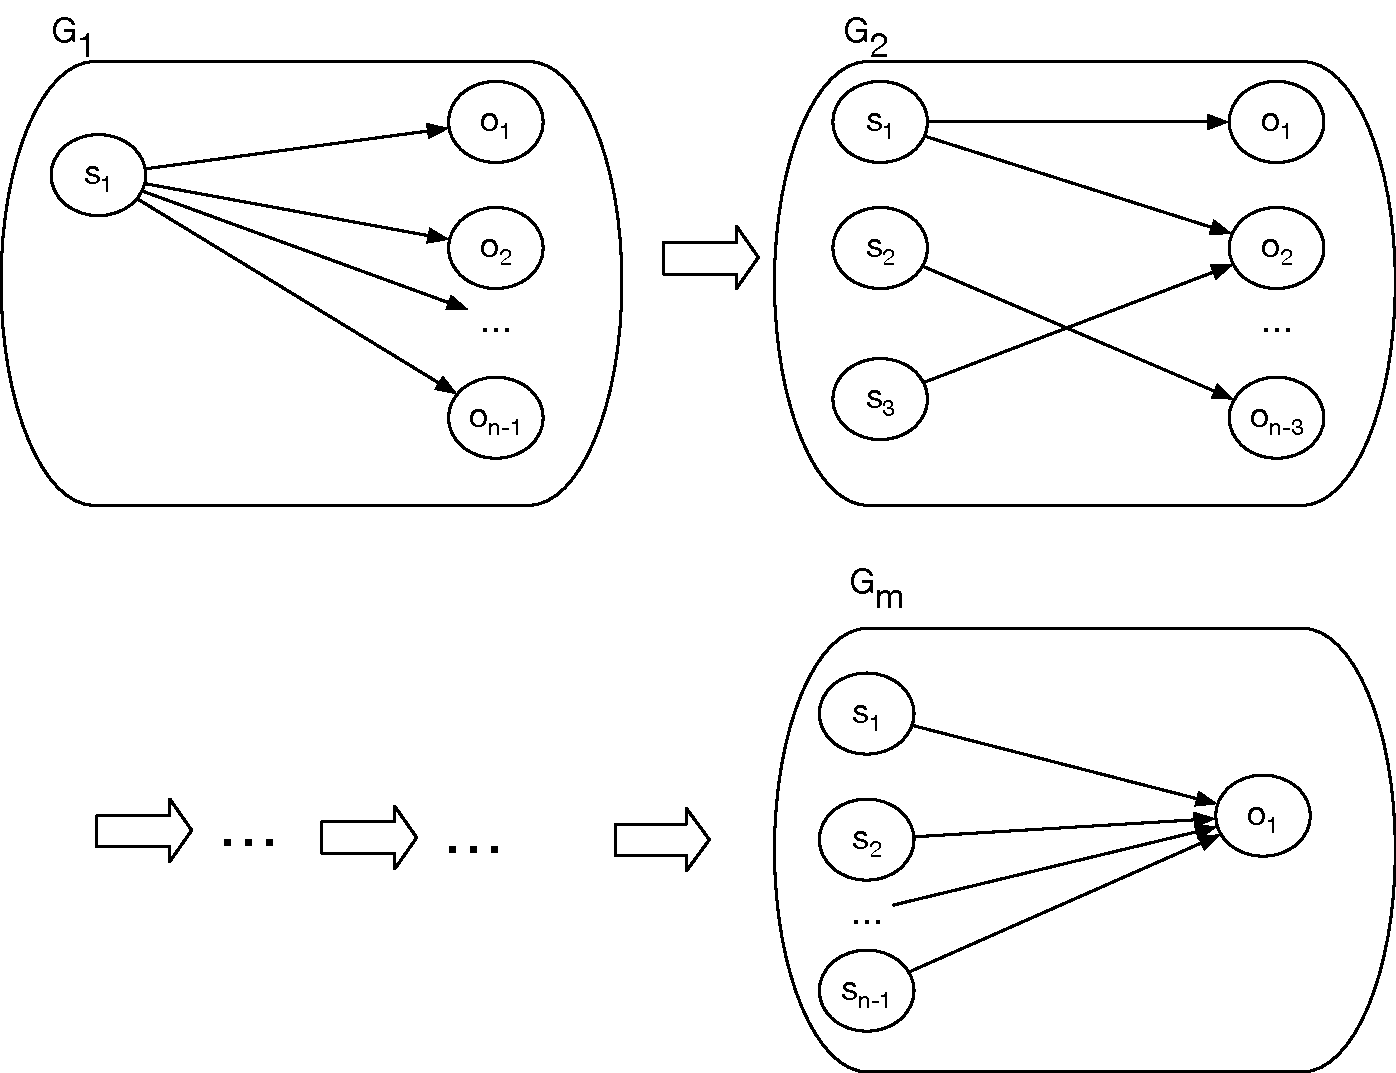
\includegraphics[width=0.8\textwidth]{figures/GRPvsHDT/starpattern.pdf}
	\caption{Step-by-step transition from hub pattern to authority pattern. The number of nodes $n$ is the same for each graph. The number of edges is also the same for each graph.}
	\label{fig:star_pattern}
\end{figure}

It is also ensured that each of the generated files has exactly the same size. This is made possible by ensuring that each URI has the same length. Since the RDF graph also has the same number of triples, the files are of the same size. Since the evaluation compares the compression ratios for the different RDF files, it is important that all files are the same size to ensure a fair comparison.

A section of such a file (for $G1$) is shown in Fig.~\ref{fig:rdfFile}. In this example, there is only one predicate for all triples. The number of predicates is always one at first. The amount of predicates has a similar effect on both compressors and is therefore omitted at first. But in Ch.~\ref{sec:evalHDT} that effect will be discussed in more detail.

Apart from that, blank nodes and literals are not used here. For both compressors, blank nodes and literals are being handled analogously to URI nodes. Therefore they are not needed at this point, in order to show the behavior of HDT and GRP in the above described scenario.

\begin{figure}[h]
	\centering
	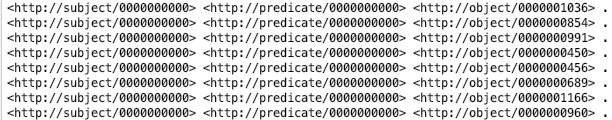
\includegraphics[width=0.8\textwidth]{figures/GRPvsHDT/file.png}
	\caption{Excerpt from the generated RDF file for $G_1$ (see Fig.~\ref{fig:star_pattern}). Each triple has the same length.}
	\label{fig:rdfFile}
\end{figure}

\section{Evaluation}\label{sec:evalHDT}

For the following evaluation HDT-Java 2.0~\footnote{\label{foot:1}https://github.com/rdfhdt/hdt-java/releases/tag/v2.0} (the currently newest version) has been used. For GRP the implementation mentioned in~\cite{maneth} has been used (written in Scala). It is not open source and has been given to us by the authors of~\cite{maneth}.

Fig.~\ref{fig:ratiosHDTWithoutDict} shows the compression ratio for HDT (without dictionary size). As expected, the ratio gets higher the more similar the graph is to the authority pattern. In general it can be said that this effect is quite small. There is only a distance of 0.002 between the minimum and the maximum. This small effect can also be seen by looking at Fig.~\ref{fig:ratiosHDTWithDict}. It can be seen that the size of the dictionary has a much bigger effect, since the compression ratio is now much larger and the curve behavior from Fig.~\ref{fig:ratiosHDTWithoutDict} is no longer recognizable. It is noticeable that the dictionary size gets bigger when the graph is further away from the star pattern. The dictionary implementation of HDT seems to be more inefficient when there are about as many subject as objects. 


\begin{figure}[h]
	\centering
	\subfloat[Without dictionary size.]{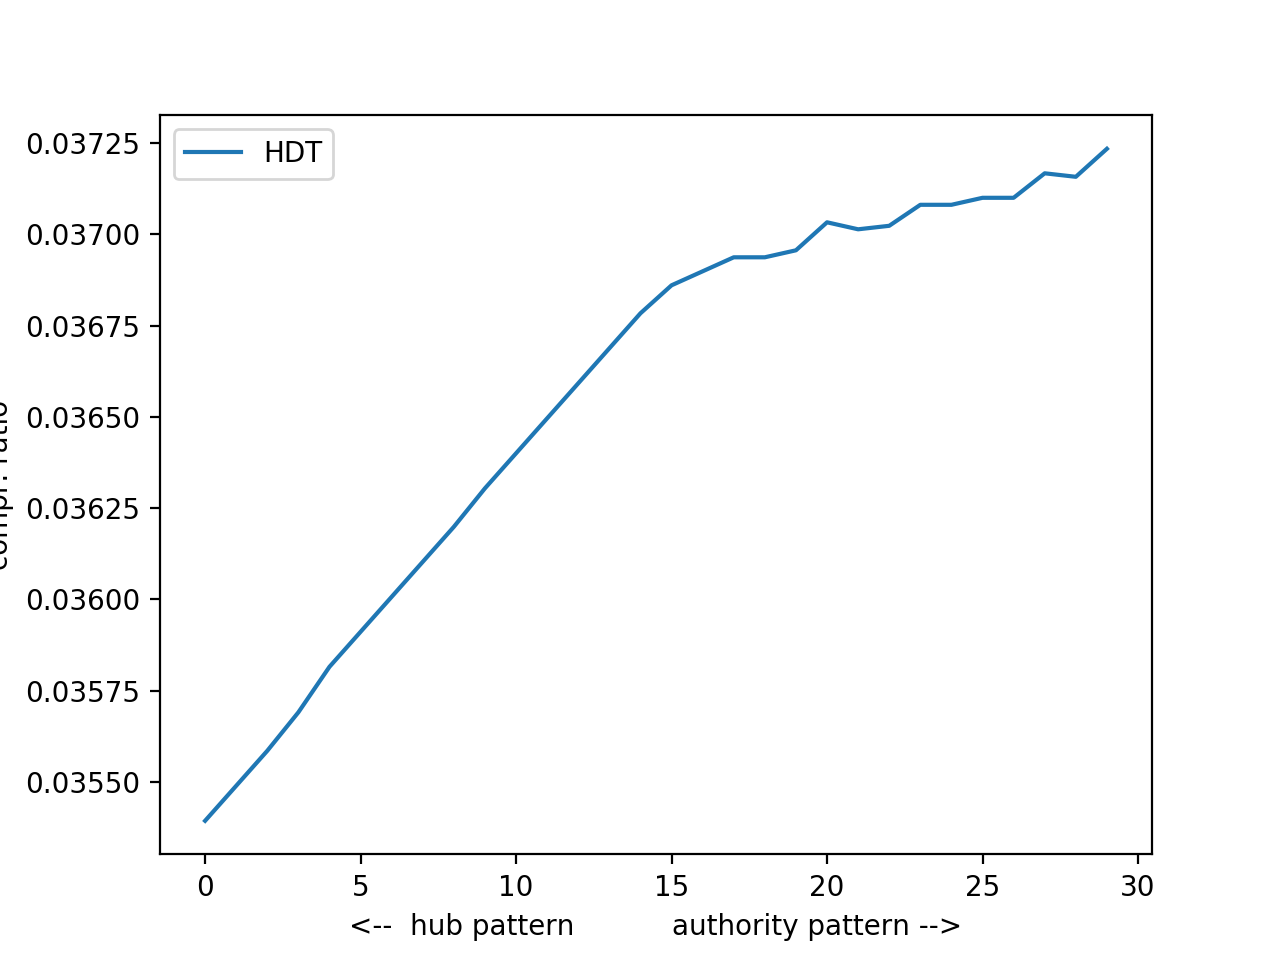
\includegraphics[width=0.5\textwidth]{figures/GRPvsHDT/hdtWithoutDict}\label{fig:ratiosHDTWithoutDict}}
	\hfill
	\subfloat[With dictionary size.]{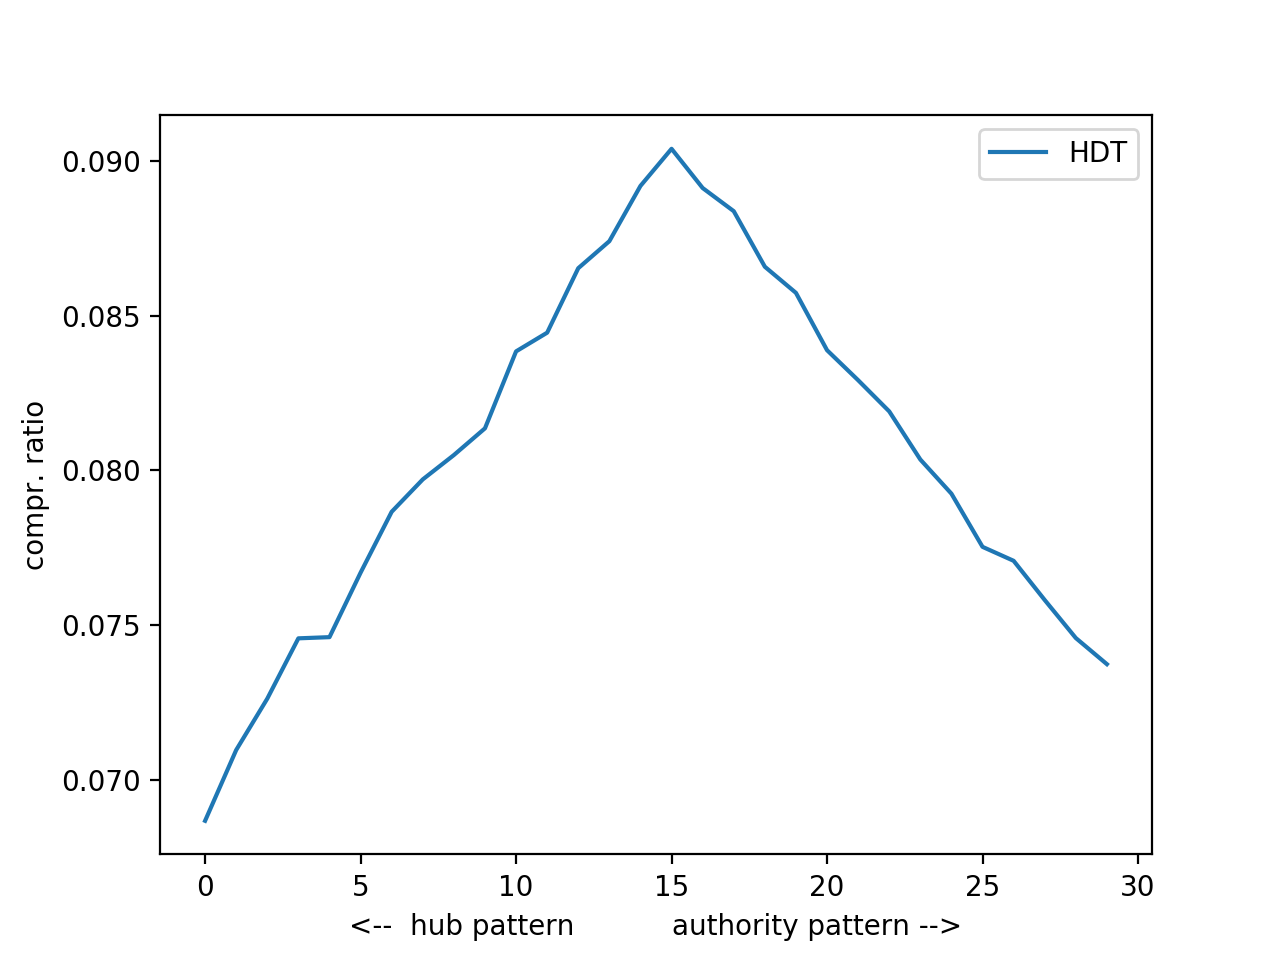
\includegraphics[width=0.5\textwidth]{figures/GRPvsHDT/hdtWithDict}\label{fig:ratiosHDTWithDict}}
	\caption{The compression ratios for HDT without and with dictionary sizes.}
\end{figure}

Next the compression ratio of GRP is considered, which is presented in Fig.~\ref{fig:ratiosGRPWithoutDict} (without dictionary sizes). Here you can see that GRP has a better compression ratio if the graph is more similar to the star pattern (hub order authority pattern). This property of GRP has also been mentioned in~\cite{maneth}. It can also be seen that the effect on the compression ratio is bigger for GRP than for HDT (standard deviation is twice as high for GRP as for HDT). A grammar-based compression is therefore more dependent on the structure of the input data.

When Fig.~\ref{fig:ratiosGRPWithDict} is considered, it can be seen that this curve behaves almost exactly like the one from Fig.~\ref{fig:ratiosHDTWithDict}, since the size of the dictionary accounts for most of the compressed data size.

\begin{figure}[h]
	\centering
	\subfloat[Without dictionary size.]{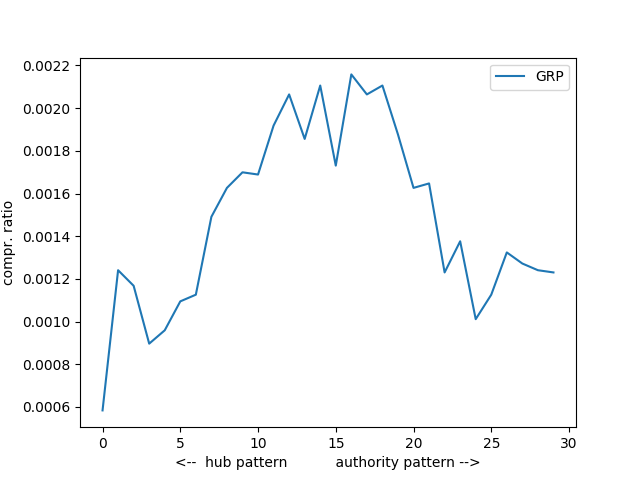
\includegraphics[width=0.5\textwidth]{figures/GRPvsHDT/grpWithoutDict}\label{fig:ratiosGRPWithoutDict}}
	\hfill
	\subfloat[With dictionary size.]{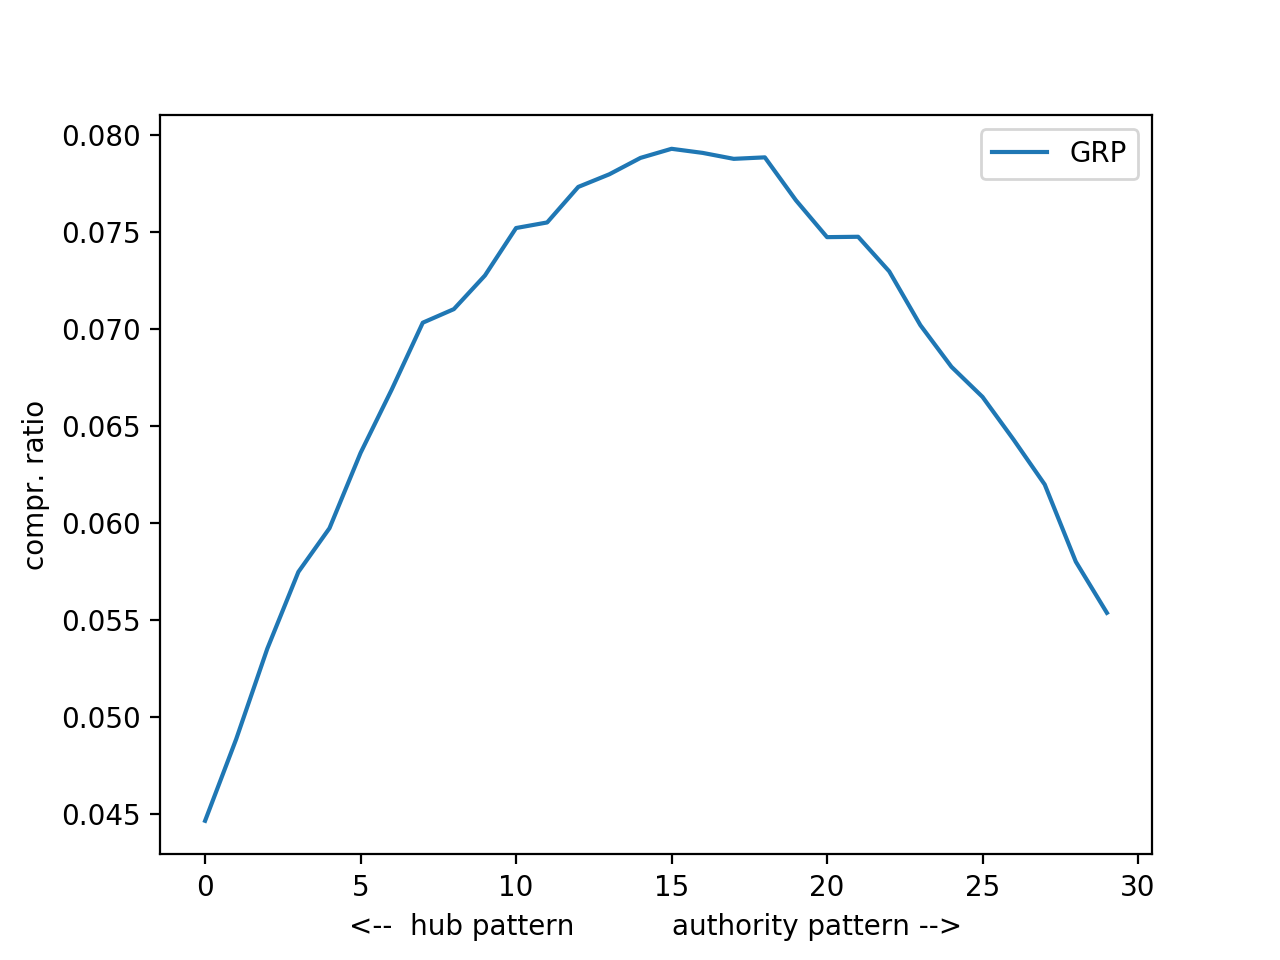
\includegraphics[width=0.5\textwidth]{figures/GRPvsHDT/grpWithDict}\label{fig:ratiosGRPWithDict}}
	\caption{The compression ratios for GRP without and with dictionary sizes.}
\end{figure}

Finally, Fig.~\ref{fig:ratiosBothWithoutDict} and Fig.\ref{fig:ratiosBothWithDict} show the compression ratios for both algorithms. Since both use the same method to compress the dictionary, the curves in Fig.~\ref{fig:ratiosBothWithDict} are very similar. However, it becomes clear that GRP compresses better than HDT. In Fig.~\ref{fig:ratiosBothWithoutDict}, the ratio of HDT is 31 times higher on average. Of course, this factor becomes much smaller in Fig.~\ref{fig:ratiosBothWithDict} because the dictionary accounts for most of the memory size. Here the compression ratio of HDT is on average 1.8 times as high as that of GRP.

\begin{figure}[h]
	\centering
	\subfloat[Without dictionary size.]{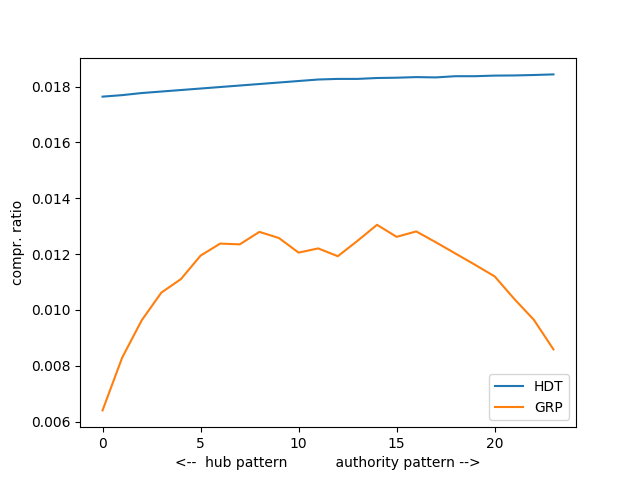
\includegraphics[width=0.5\textwidth]{figures/GRPvsHDT/bothWithoutDict}\label{fig:ratiosBothWithoutDict}}
	\hfill
	\subfloat[With dictionary size.]{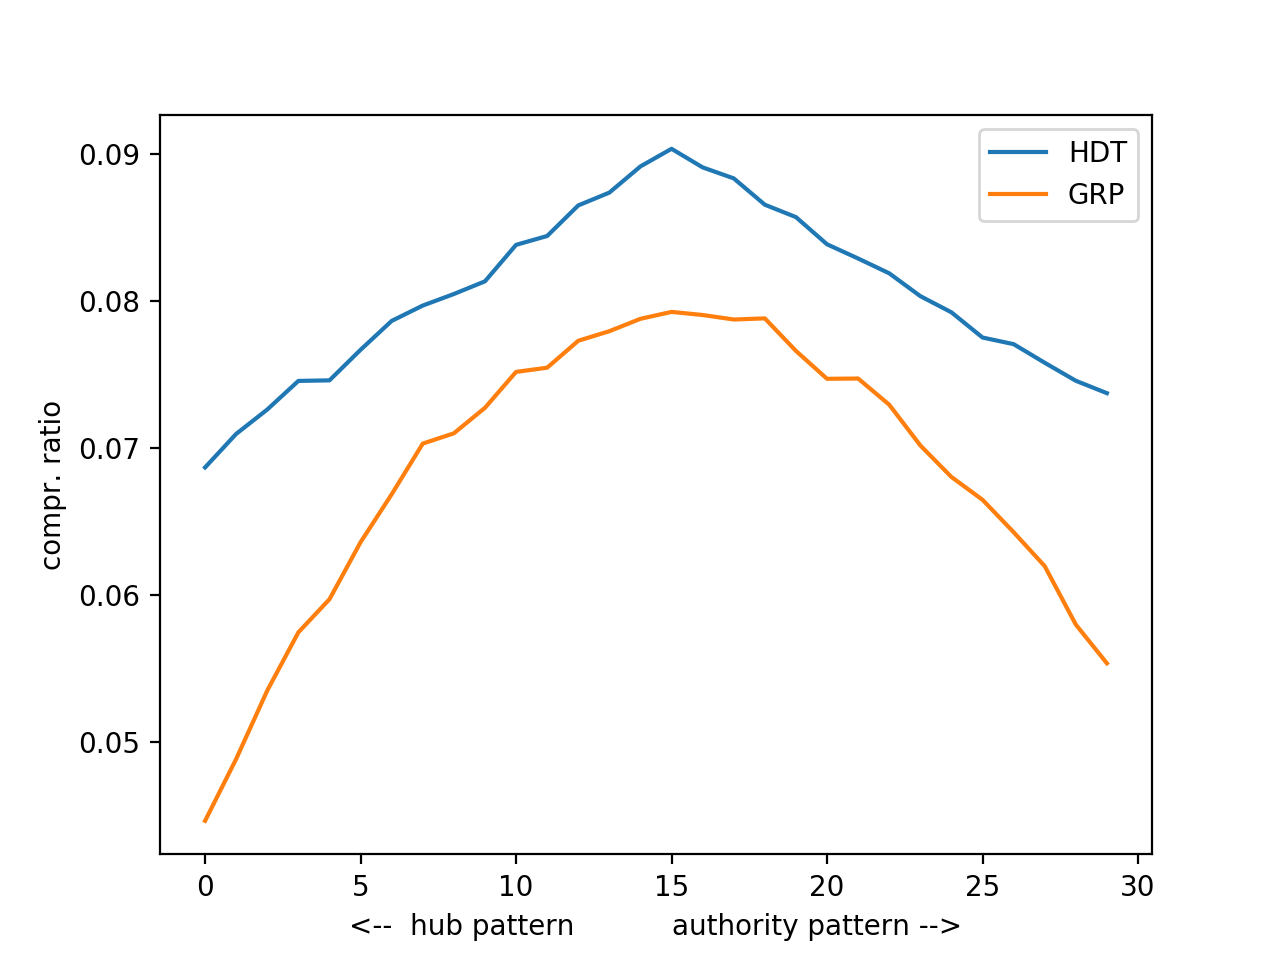
\includegraphics[width=0.5\textwidth]{figures/GRPvsHDT/bothWithDict}\label{fig:ratiosBothWithDict}}
	\caption{The compression ratios for GRP and HDT without and with dictionary sizes.}
\end{figure}

One could now argue that only one distinct predicate was used in that scenario and this is beneficial for GRP, as it gets worse as the number of predicates increases. Therefore a further evaluation is made in Fig.~\ref{fig:bothwithdict1000predicates}, where 1000 distinct predicates have been used. That is a quite high number considering the number of triples (1199) compared to real RDF data \todo{belegen}. One can see that the compression ratios are now higher for both compressors, but still GRP's ratio is always smaller than HDT's. HDT's ratio is still 1.7 times higher on average. So, the increasing number of predicates has a similar effect on both algorithms.

\begin{figure}
	\centering
	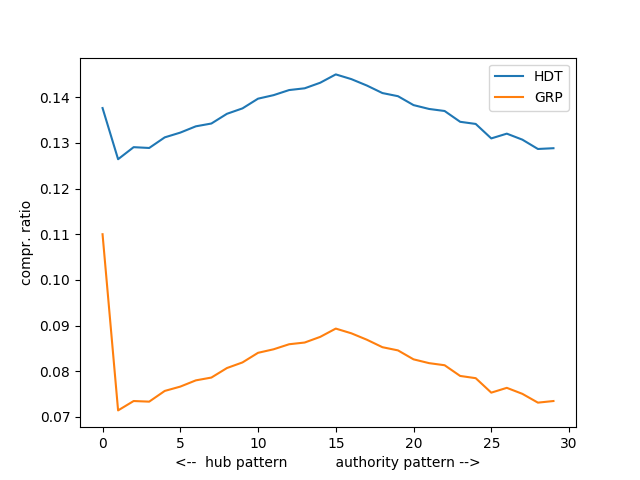
\includegraphics[width=0.7\linewidth]{figures/GRPvsHDT/bothWithDict1000Predicates}
	\caption{The compression ratios for GRP and HDT with dictionary sizes. Graphs have now 1000 distinct predicates.}
	\label{fig:bothwithdict1000predicates}
\end{figure}

Apart from the compression ratio, the run time is also important for the overall performance. Fig.~\ref{fig:runtimes} shows the average run times of the two algorithms. For this the same scenario with the star pattern (and only one distinct predicate) was used. It has been executed 100 times to get a sophisticated run time measurement, because the run time also depends on the current CPU workload of the computer.

\begin{figure}
	\centering
	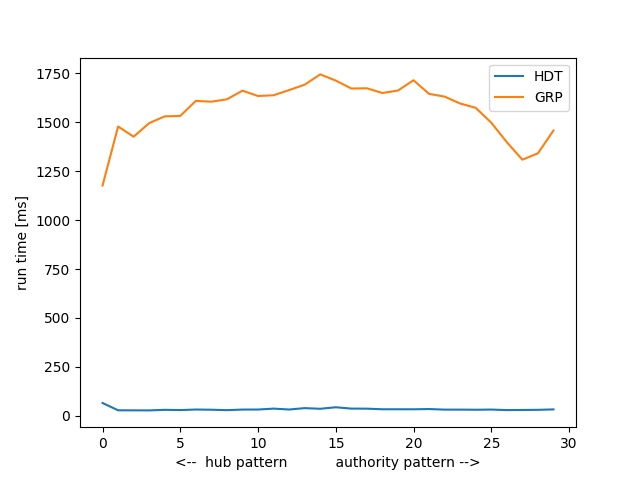
\includegraphics[width=0.7\linewidth]{figures/GRPvsHDT/runtimes}
	\caption{Run times of both algorithms (average run time of 100 consecutive executions).}
	\label{fig:runtimes}
\end{figure}


It can be seen that the runtime of GRP is significantly higher than that of GRP. It is on average ca. 48 times as high.

However, it should also be noted that the implementation of GRP is rather rudimentary  (according to the authors of~\cite{maneth}), while that of HDT has been under development for some time. So they are not comparable in terms of quality. Unfortunately, one cannot say at this point whether a more professional implementation of GRP will also be slower than HDT.

In addition one can notice that GRP's run time fluctuates more than that of HDT. GRP has a standard deviation of about 134, while HDT only has a standard deviation of about 7. One reason for this is that GRP, in contrast to HDT, is non-deterministic because of the partly random search order of the graph. On the other hand, the high deviations are also a confirmation of the above mentioned hypothesis that the behavior of GRP depends more on the structure of the input data than HDT does.
























\chapter{Implementation}
\label{ch:implementation}




\chapter{Evaluation}
\label{ch:evaluation}





\chapter{Summary and Discussion}
\label{ch:summary_and_discussion}
discussion



%\cleardoublepage
%\phantomsection
%\addcontentsline{toc}{chapter}{\listfigurename}
\listoffigures
\listoftables

\chapter*{List of Acronyms}
\begin{acronym}[ICANN]
	\acro{RDF}{Resource Description Framework}
	\acro{HDT}{Header Dictionary Triples}
	\acro{GRP}{GraphRePair}
	\acro{RDFS}{RDF Schema}
	\acro{OWL}{Web Ontology Language}
	\acro{$ CR_C $}{Compression Ratio for Compressor $C$}
	\acro{$ CT_C $}{Compression Run Time for Compressor $C$}
	\acro{$ DCT_C $}{Decompression Run Time for Compressor $C$}
	\acro{$ ELR $}{Edge Label Ratio}
	\acro{$ SPS $}{Star Pattern Similarity}
	\acro{$ IER $}{Input Edge Ratio}
	\acro{$ OER $}{Output Edge Ratio}
	\acro{$ SR $}{Size Ratio}
\end{acronym}





% include the bibliography, and add it as a chapter the table of contents
\newpage
\addcontentsline{toc}{chapter}{Bibliography}
\bibliographystyle{alpha}
\bibliography{literature.bib}


%%%%%%%%%
% the appendices of your thesis go into file appendix.tex
%%%%%%%%%
\appendix



\end{document}
